\documentclass[12pt,a4paper,twoside]{report}
% -------------------------------------------------------------------- %
% Pacotes

\usepackage[utf8]{inputenc}
\usepackage[T1]{fontenc}
\usepackage[brazil]{babel}
\usepackage[fixlanguage]{babelbib}
\usepackage[pdftex]{graphicx}      % usamos arquivos pdf/png como figuras
\usepackage{setspace}              % espaçamento flexvel
\usepackage{indentfirst}           % indentação do primeiro parágrafo
\usepackage{makeidx}               % índice remissivo
\usepackage[nottoc]{tocbibind}     % acrescentamos a bibliografia/indice/conteudo no Table of Contents
\usepackage{courier}               % usa o Adobe Courier no lugar de Computer Modern Typewriter
\usepackage{type1cm}               % fontes realmente escaláveis
\usepackage{titletoc}
\usepackage{ucs}
\usepackage[font=small,format=plain,labelfont=bf,up,textfont=it,up]{caption}
\usepackage[usenames,svgnames,dvipsnames]{xcolor}
\usepackage[a4paper,top=2.54cm,bottom=2.0cm,left=2.0cm,right=2.54cm]{geometry} % margens
\usepackage{amsmath}
\usepackage{booktabs} % cria tabelas em formato profissional
\usepackage[pdftex,plainpages=false,pdfpagelabels,pagebackref,colorlinks=true,citecolor=DarkGreen,
linkcolor=NavyBlue,urlcolor=DarkRed,filecolor=green,bookmarksopen=true]{hyperref} % links coloridos
\usepackage[all]{hypcap}                % soluciona o problema com o hyperref e capítulos
\usepackage[square,sort,nonamebreak,comma]{natbib}  % citação bibliográfica alpha
\fontsize{60}{62}\usefont{OT1}{cmr}{m}{n}{\selectfont}
\usepackage{upquote}                    % formata apóstrofes '
\usepackage{textcomp}

% Para formatar corretamente as URLs
\usepackage{url}
% -------------------------------------------------------------------- %
% Cabeçalhos similares ao TAOCP de Donald E. Knuth
\usepackage{fancyhdr}
\pagestyle{fancy}
\fancyhf{}
\renewcommand{\chaptermark}[1]{\markboth{\MakeUppercase{#1}}{}}
\renewcommand{\sectionmark}[1]{\markright{\MakeUppercase{#1}}{}}
\renewcommand{\headrulewidth}{0pt}

\frenchspacing                     % arruma o espaço: id est (i.e.) e exempli gratia (e.g.)
\urlstyle{same}                    % URL com o mesmo estilo do texto e no mono-spaced
\makeindex                         % para o índice remissivo
\raggedbottom                      % para no permitir espaços extras no texto
\fontsize{60}{62}\usefont{OT1}{cmr}{m}{n}{\selectfont}
\cleardoublepage
\normalsize

% -------------------------------------------------------------------- %
% Cores para formatação de código
\usepackage{color}
\definecolor{vermelho}{rgb}{0.6,0,0} % para strings
\definecolor{verde}{rgb}{0.25,0.5,0.35} % para comentários
\definecolor{roxo}{rgb}{0.5,0,0.35} % para palavras-chaves
\definecolor{azul}{rgb}{0.25,0.35,0.75} % para strings
\definecolor{cinza-claro}{gray}{0.95}
% -------------------------------------------------------------------- %
% Opções de listagem usados para o código fonte
% Ref: http://en.wikibooks.org/wiki/LaTeX/Packages/Listings
\usepackage{listings}           % para formatar código-fonte (ex. em Java)

\lstset{ %
language=Python,                      % seleciona a linguagem do código
basicstyle=\footnotesize\ttfamily,    % o tamanho da fonte usado no código
commentstyle=\color{verde}\bfseries,  % formatação de comentários
stringstyle=\color{azul},             % formatação de strings
upquote=true,
numbers=left,                   % onde colocar os números de linha
numberstyle=\tiny,  % o tamanho da fonte usada para a numeração das linhas
stepnumber=1,                   % o intervalo entre dois números de linhas. Se for 1, numera cada uma.
numbersep=5pt,                  % how far the line-numbers are from the code
showspaces=false,               % show spaces adding particular underscores
showstringspaces=false,         % underline spaces within strings
showtabs=false,                 % show tabs within strings adding particular underscores
keywordstyle=\color{roxo}\bfseries,
keywordstyle=[1]\color{roxo}\bfseries,
keywordstyle=[2]\color{verde}\bfseries,
frame=b,                   % adds a frame around the code
framerule=0.6pt,
tabsize=2,                      % sets default tabsize to 2 spaces
captionpos=t,                   % sets the caption-position to top
breaklines=true,                % sets automatic line breaking
breakatwhitespace=false,        % sets if automatic breaks should only happen at whitespace
escapeinside={\%*}{*)},         % if you want to add a comment within your code
backgroundcolor=\color[rgb]{1.0,1.0,1.0}, % choose the background color.
rulecolor=\color[rgb]{0.8,0.8,0.8},
extendedchars=true,
xleftmargin=10pt,
xrightmargin=10pt,
framexleftmargin=10pt,
framexrightmargin=10pt,
literate={â}{{\^{a}}}1  % para formatar corretamente os acentos do Português ao usar utf8
    {ê}{{\^{e}}}1
    {ô}{{\^{o}}}1
    {Â}{{\^{A}}}1
    {Ê}{{\^{E}}}1
    {Ô}{{\^{O}}}1
    {á}{{\'{a}}}1
    {é}{{\'{e}}}1
    {í}{{\'{i}}}1
    {ó}{{\'{o}}}1
    {ú}{{\'{u}}}1
    {Á}{{\'{A}}}1
    {É}{{\'{E}}}1
    {Í}{{\'{I}}}1
    {Ó}{{\'{O}}}1
    {Ú}{{\'{U}}}1
    {à}{{\`{a}}}1
    {À}{{\`{A}}}1
    {ã}{{\~{a}}}1
    {õ}{{\~{o}}}1
    {Ã}{{\~{A}}}1
    {Õ}{{\~{O}}}1
    {ç}{{\c{c}}}1
    {Ç}{{\c{C}}}1
    {ü}{{\"u}}1
    {Ü}{{\"U}}1
}

\renewcommand{\lstlistingname}{Listagem}
\renewcommand{\lstlistlistingname}{Lista de Listagens}

% \captionsetup[lstlisting]{singlelinecheck=false, labelfont={blue}, textfont={blue}}
\usepackage{caption}
\DeclareCaptionFont{white}{\color{white}}
\DeclareCaptionFormat{listing}{\colorbox[cmyk]{0.43, 0.35, 0.35,0.01}{\parbox{\textwidth}{\hspace{15pt}#1#2#3}}}
\captionsetup[lstlisting]{format=listing,labelfont=white,textfont=white, singlelinecheck=false, margin=0pt, font={bf,footnotesize}}

\title{Análise experimental de algoritmos usando Python}
\author{Patrícia Mariana Ramos Marcolino\\
\texttt{\small \url{pmrmarcolino@hotmail.com}}
\vspace{1cm} \\
Eduardo Pinheiro Barbosa \\
\texttt{\small \url{eduardptu@hotmail.com}}
\vspace{1cm} \\
Faculdade de Computação \\
Universidade Federal de Uberlândia
}
\date{\today}

\begin{document}
\maketitle
% -------------------------------------------------------------------- %
% Listas de figuras, tabelas e códigos criadas automaticamente
\listoffigures
\listoftables
\lstlistoflistings
% -------------------------------------------------------------------- %

% -------------------------------------------------------------------- %
% Sumário
\tableofcontents
% cabeçalho para as páginas de todos os capítulos
\fancyhead[RE,LO]{\thesection}

%\singlespacing              % espaçamento simples
\setlength{\parskip}{0.15in} % espaçamento entre paragráfos

\chapter{Análise}

O algoritmo Radix Sort ordena um vetor A de n números inteiros
com um número constante d de dígitos, através de ordenações
parciais dígito a dígito.\\
Podemos também ordenar os números ordenando-os segundo
cada um de seus dígitos, começando pelo menos significativo.\\
O seguinte argumento indutivo garante a corretude do algoritmo:\\
Por hipótese de indução, assumimos que os números estão
ordenados com relação aos $i - 1$ dígitos menos
significativos.\\
Ordenando os números com relação ao i-ésimo dígito, com um
algoritmo estável, teremos então os números ordenados com
relação aos i dígitos menos significativos, pois:
\\Para dois números com o i-ésimo dígito distintos, o de menor valor
no dígito estará antes do de maior valor;
\\E se ambos possuem o i -ésimo dígito igual, então a ordem dos
dois também estará correta pois utilizamos um método de
ordenação estável e, por hipótese de indução, os dois elementos já
estavam ordenados segundo os i-1dígitos menos significativos.
A complexidade do Radix Sort depende da complexidade
do algoritmo estável usado para ordenar cada dígito dos
elementos.
Se essa complexidade estiver em $\theta(f(n))$, obtemos uma
complexidade total de $\theta(d f(n))$ para o Radix Sort.
Como supomos d constante, a complexidade reduz-se para
$\theta(f(n))$.
Se o algoritmo estável for, por exemplo, o Counting Sort,
obtemos a complexidade $\theta(n + k)$.
Supondo $k ∈ O(n)$, resulta numa complexidade linear em n.
Em contraste, um algoritmo por comparação como o
MergeSort teria complexidade $n \log(n)$.
Assim, o Radix Sort é mais vantajoso que o MergeSort
quando $d < \log(n)$, ou seja, o número de dígitos for menor
que log n.\\
Se considerarmos que n também é um limite superior para
o maior valor a ser ordenado, então $O(\log (n))$ é uma
estimativa para o tamanho, em dígitos, desse número.
\\
Veja que se o uso de memória auxiliar for muito limitado,
então o melhor mesmo é usar um algoritmo de ordenação
por comparação in-place.\\
Note que e possível usar o Radix Sort para ordenar outros
tipos de elementos, como datas, palavras em ordem
lexicográfica e qualquer outro tipo que possa ser visto como
uma tupla ordenada de itens comparáveis

\chapter{Resultados}
\section{Tabelas}

\begin{table}[ht]
\centering
\begin{tabular}{rrr} \toprule
        n &    comparações &       tempo(s) \\ \midrule
      32  &              7 &      0.001504 \\
      64  &              7 &      0.002867 \\
     128  &              7 &      0.005680 \\
     256  &              7 &      0.011012 \\
     512  &              7 &      0.022024 \\
    1024  &              7 &      0.043471 \\
    2048  &              7 &      0.086574 \\
    4096  &              7 &      0.172890 \\
    8192  &              7 &      0.356761 \\
\bottomrule\addlinespace
\end{tabular}
\caption{Tabela com vetor teste aleatório: A linha te interesse analisada para este caso é a 16.}
\label{tab:radixsortAleatorio}
\end{table}


\begin{figure}[ht]
\centering 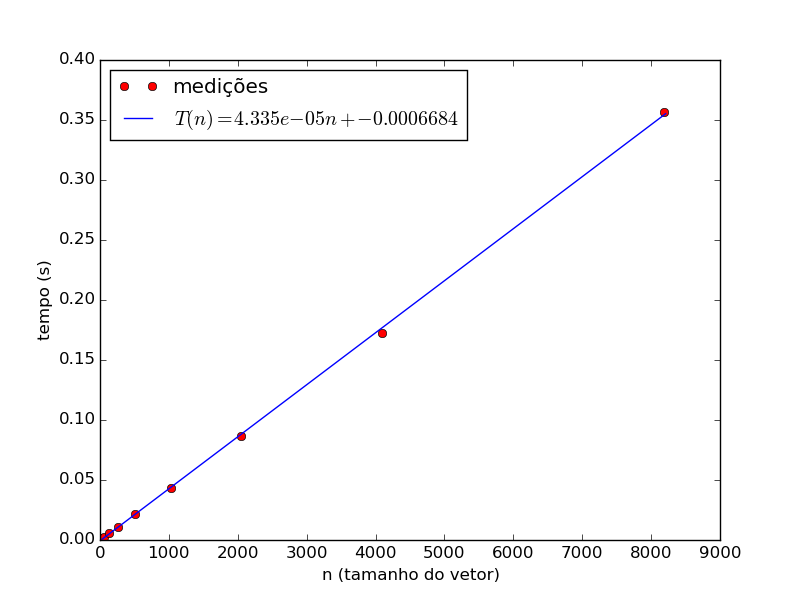
\includegraphics[scale=0.8]{../radixsort/imagens/radixsortAleatorio0.png}
\caption{A análise do grafico para $2^{32}$ segue abaixo para radixsort}

Tendo a função $T(n) = 4.335\mathrm{e}-5*n-0.0006684$ e para o $n =2^{32}$, $T(2^{32}) =186186.8316132
$ 
\label{fig:radixsortAleatorio0}
\end{figure}

\begin{figure}[ht]
\centering 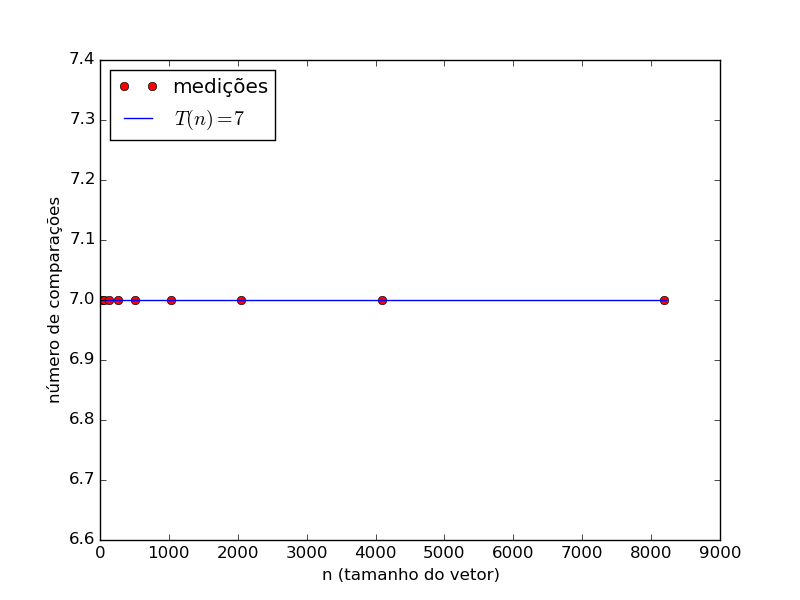
\includegraphics[scale=0.8]{../radixsort/imagens/radixsortAleatorio1.png}
\caption{A análise do grafico para $2^{32}$ segue abaixo para radixsort}

Tendo a função $T(n) = 7$ e para o $n =2^{32}$, $T(2^{32}) = 7$
\label{fig:radixsortAleatorio1}
\end{figure}


\begin{table}[ht]
\centering
\begin{tabular}{rrr} \toprule
        n &    comparações &       tempo(s) \\ \midrule
      32  &              7 &      0.001576 \\
      64  &              7 &      0.002985 \\
     128  &              7 &      0.005884 \\
     256  &              7 &      0.011169 \\
     512  &              7 &      0.022276 \\
    1024  &              7 &      0.043654 \\
    2048  &              7 &      0.084924 \\
    4096  &              7 &      0.170405 \\
    8192  &              7 &      0.352600 \\
\bottomrule\addlinespace
\end{tabular}
\caption{Tabela com vetor teste crescente: A linha te interesse analisada para este caso é a 16.}
\label{tab:radixsortCrescente}
\end{table}


\begin{figure}[ht]
\centering 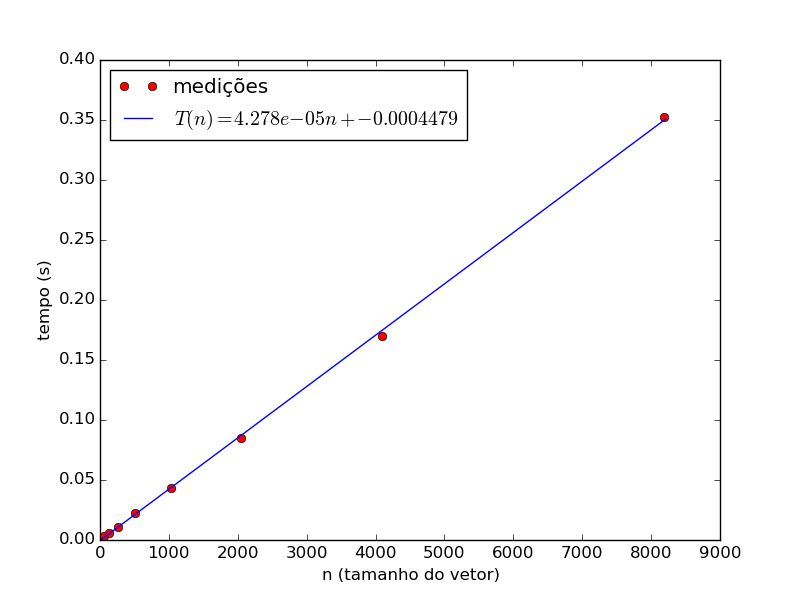
\includegraphics[scale=0.8]{../radixsort/imagens/radixsortCrescente0.png}
\caption{A análise do grafico para $2^{32}$ segue abaixo para radixsort}

Tendo a função $T(n) = 4.278\mathrm{e}-5*n-0.0004479$ e para o $n =2^{32}$, $T(2^{32}) = 183738.70047498$
\label{fig:radixsortCrescente0}
\end{figure}

\begin{figure}[ht]
\centering 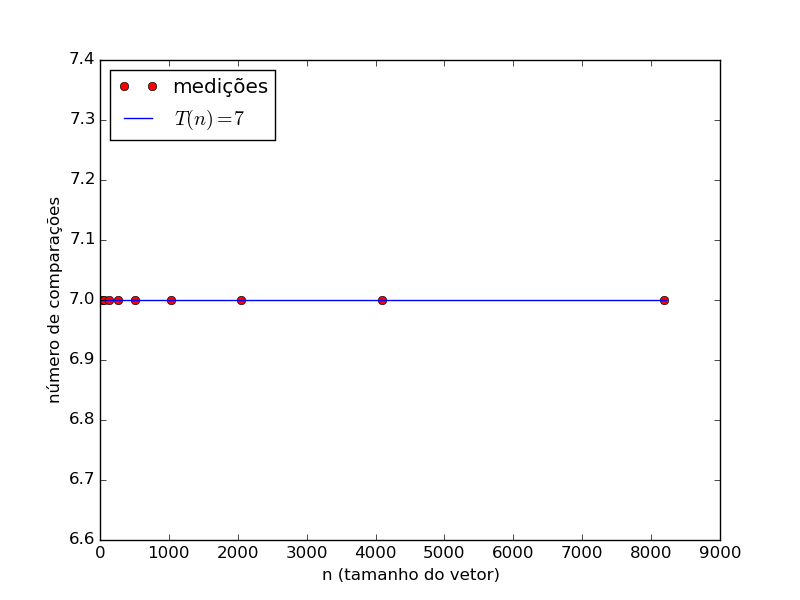
\includegraphics[scale=0.8]{../radixsort/imagens/radixsortCrescente1.png}
\caption{A análise do grafico para $2^{32}$ segue abaixo para radixsort}

Tendo a função $T(n) = 7$ e para o $n =2^{32}$, $T(2^{32}) =7$
\label{fig:radixsortCrescente1}
\end{figure}


\begin{table}[ht]
\centering
\begin{tabular}{rrr} \toprule
        n &    comparações &       tempo(s) \\ \midrule
      32  &              7 &      0.001467 \\
      64  &              7 &      0.002939 \\
     128  &              7 &      0.005533 \\
     256  &              7 &      0.010907 \\
     512  &              7 &      0.022306 \\
    1024  &              7 &      0.043331 \\
    2048  &              7 &      0.083704 \\
    4096  &              7 &      0.177603 \\
    8192  &              7 &      0.363321 \\
\bottomrule\addlinespace
\end{tabular}
\caption{Tabela com vetor teste decrescente: A linha te interesse analisada para este caso é a 16.}
\label{tab:radixsortDecrescente}
\end{table}


\begin{figure}[ht]
\centering 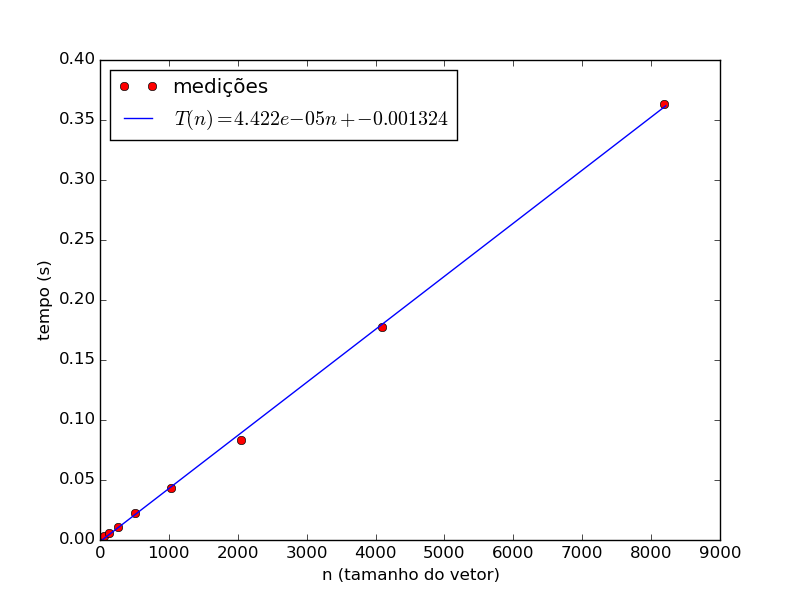
\includegraphics[scale=0.8]{../radixsort/imagens/radixsortDecrescente0.png}
\caption{A análise do grafico para $2^{32}$ segue abaixo para radixsort}

Tendo a função $T(n) = 4.422\mathrm{e}-5*n-0.0001324$ e para o $n =2^{32}$, $T(2^{32}) = 189923.45369672$
\label{fig:radixsortDecrescente0}
\end{figure}

\begin{figure}[ht]
\centering 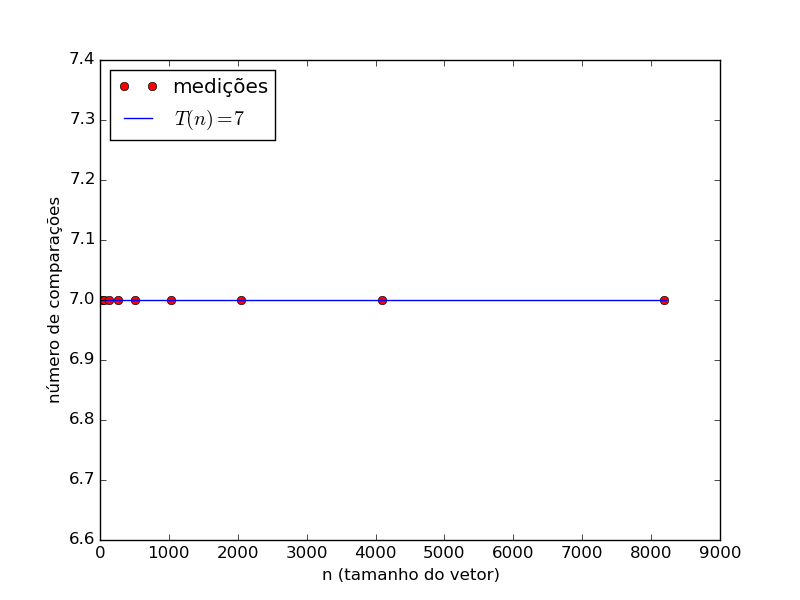
\includegraphics[scale=0.8]{../radixsort/imagens/radixsortDecrescente1.png}
\caption{A análise do grafico para $2^{32}$ segue abaixo para radixsort}

Tendo a função $T(n) = 7$ e para o $n =2^{32}$, $T(2^{32}) =7$
\label{fig:radixsortDecrescente1}
\end{figure}


\begin{table}[ht]
\centering
\begin{tabular}{rrr} \toprule
        n &    comparações &       tempo(s) \\ \midrule
      32  &              7 &      0.001560 \\
      64  &              7 &      0.002925 \\
     128  &              7 &      0.005988 \\
     256  &              7 &      0.011510 \\
     512  &              7 &      0.024760 \\
    1024  &              7 &      0.042652 \\
    2048  &              7 &      0.085191 \\
    4096  &              7 &      0.177059 \\
    8192  &              7 &      0.370108 \\
\bottomrule\addlinespace
\end{tabular}
\caption{Tabela com vetor teste quase crecente 10\%: A linha te interesse analisada para este caso é a 16.}
\label{tab:radixsortQuaseCresc10}
\end{table}


\begin{figure}[ht]
\centering 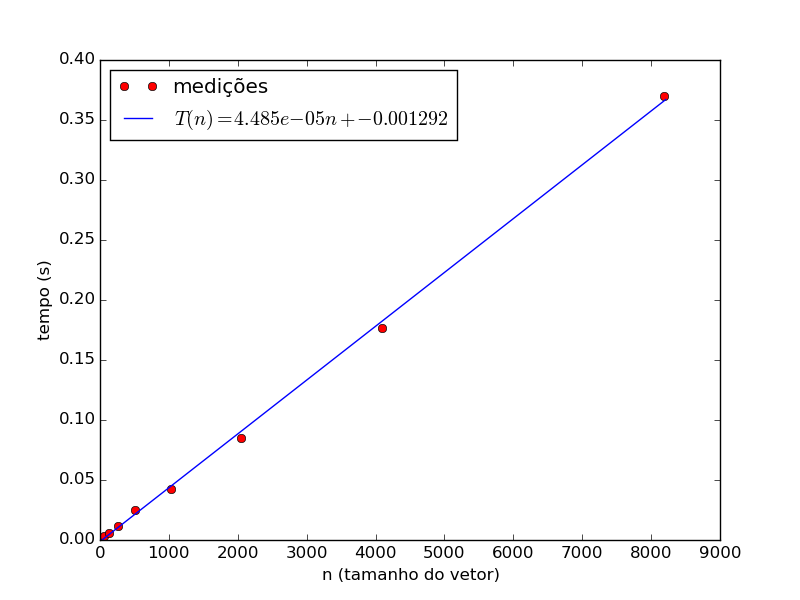
\includegraphics[scale=0.8]{../radixsort/imagens/radixsortQuaseCresc100.png}
\caption{A análise do grafico para $2^{32}$ segue abaixo para radixsort}

Tendo a função $T(n) = 4.485\mathrm{e}-5*n-0.0001292$ e para o $n =2^{32}$, $T(2^{32}) =192629.2830964$
\label{fig:radixsortQuaseCresc100}
\end{figure}

\begin{figure}[ht]
\centering 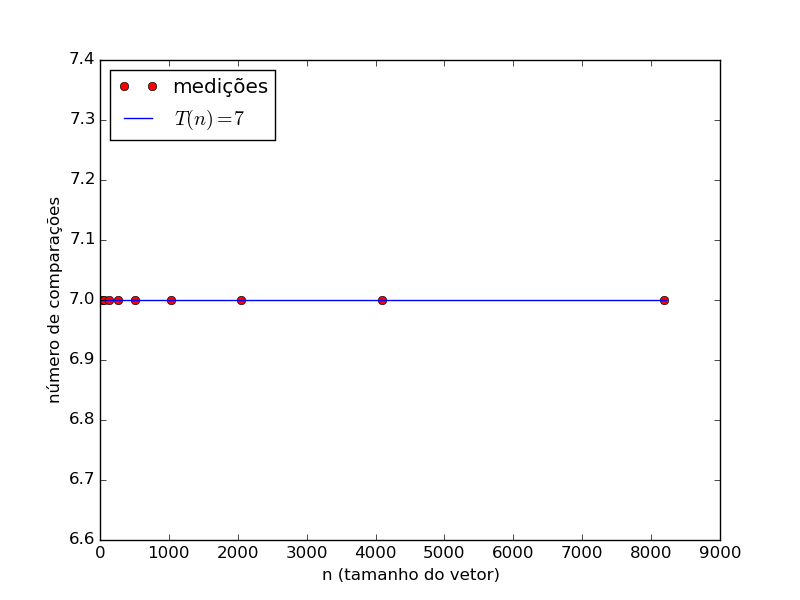
\includegraphics[scale=0.8]{../radixsort/imagens/radixsortQuaseCresc101.png}
\caption{A análise do grafico para $2^{32}$ segue abaixo para radixsort}

Tendo a função $T(n) = 7$ e para o $n =2^{32}$, $T(2^{32}) = 7$
\label{fig:radixsortQuaseCresc101}
\end{figure}


\begin{table}[ht]
\centering
\begin{tabular}{rrr} \toprule
        n &    comparações &       tempo(s) \\ \midrule
      32  &              7 &      0.001606 \\
      64  &              7 &      0.002909 \\
     128  &              7 &      0.005773 \\
     256  &              7 &      0.011253 \\
     512  &              7 &      0.022697 \\
    1024  &              7 &      0.045749 \\
    2048  &              7 &      0.087966 \\
    4096  &              7 &      0.176329 \\
    8192  &              7 &      0.352703 \\
\bottomrule\addlinespace
\end{tabular}
\caption{Tabela com vetor teste quase crecente 20\%: A linha te interesse analisada para este caso é a 16.}
\label{tab:radixsortQuaseCresc20}
\end{table}


\begin{figure}[ht]
\centering 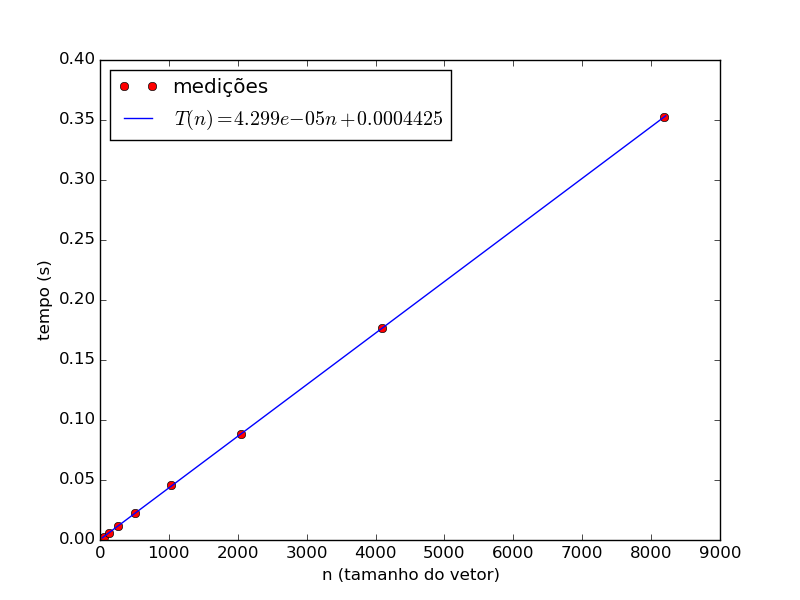
\includegraphics[scale=0.8]{../radixsort/imagens/radixsortQuaseCresc200.png}
\caption{A análise do grafico para $2^{32}$ segue abaixo para radixsort}

Tendo a função $T(n) = 4.299\mathrm{e}-5*n-0.0004425$ e para o $n =2^{32}$, $T(2^{32}) =184640.64361254$
\label{fig:radixsortQuaseCresc200}
\end{figure}

\begin{figure}[ht]
\centering 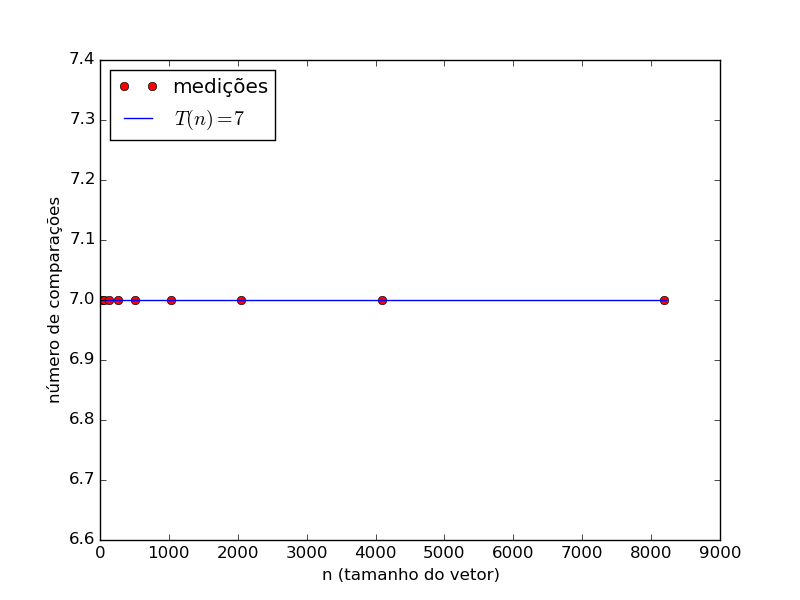
\includegraphics[scale=0.8]{../radixsort/imagens/radixsortQuaseCresc201.png}
\caption{A análise do grafico para $2^{32}$ segue abaixo para radixsort}

Tendo a função $T(n) = 7$ e para o $n =2^{32}$, $T(2^{32}) =7$
\label{fig:radixsortQuaseCresc201}
\end{figure}

\clearpage
\begin{table}[ht]
\centering
\begin{tabular}{rrr} \toprule
        n &    comparações &       tempo(s) \\ \midrule
      32  &              7 &      0.001494 \\
      64  &              7 &      0.002827 \\
     128  &              7 &      0.005499 \\
     256  &              7 &      0.010844 \\
     512  &              7 &      0.022666 \\
    1024  &              7 &      0.042608 \\
    2048  &              7 &      0.084882 \\
    4096  &              7 &      0.170542 \\
    8192  &              7 &      0.344394 \\
\bottomrule\addlinespace
\end{tabular}
\caption{Tabela com vetor teste quase crecente 30\%: A linha te interesse analisada para este caso é a 16.}
\label{tab:radixsortQuaseCresc30}
\end{table}


\begin{figure}[ht]
\centering 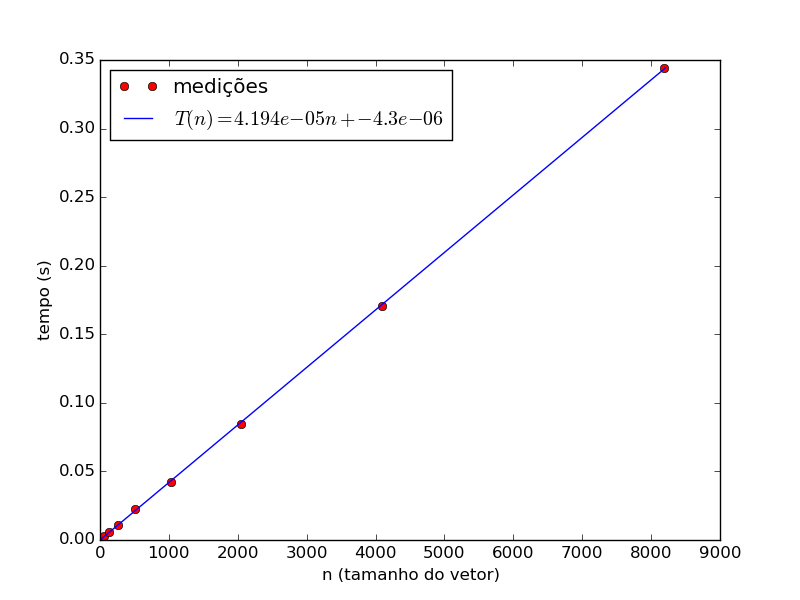
\includegraphics[scale=0.8]{../radixsort/imagens/radixsortQuaseCresc300.png}
\caption{A análise do grafico para $2^{32}$ segue abaixo para radixsort}

Tendo a função $T(n) = 4.194\mathrm{e}-5*n-4.3\mathrm{e}-6$ e para o $n =2^{32}$, $T(2^{32}) = 180130.92838994$
\label{fig:radixsortQuaseCresc300}
\end{figure}

\begin{figure}[ht]
\centering 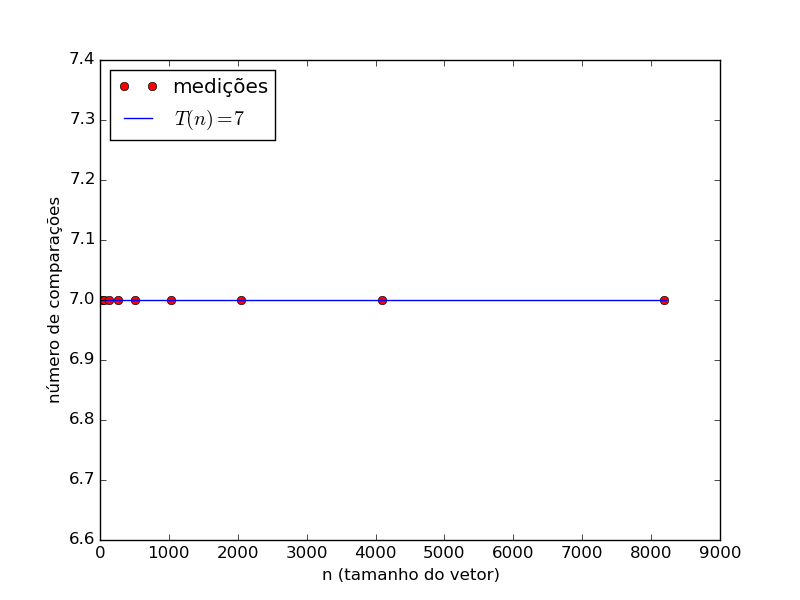
\includegraphics[scale=0.8]{../radixsort/imagens/radixsortQuaseCresc301.png}
\caption{EA análise do grafico para $2^{32}$ segue abaixo para radixsort}

Tendo a função $T(n) = 7$ e para o $n =2^{32}$, $T(2^{32}) = 7$
\label{fig:radixsortQuaseCresc301}
\end{figure}


\begin{table}[ht]
\centering
\begin{tabular}{rrr} \toprule
        n &    comparações &       tempo(s) \\ \midrule
      32  &              7 &      0.001515 \\
      64  &              7 &      0.003014 \\
     128  &              7 &      0.005460 \\
     256  &              7 &      0.011347 \\
     512  &              7 &      0.022346 \\
    1024  &              7 &      0.043654 \\
    2048  &              7 &      0.088364 \\
    4096  &              7 &      0.173760 \\
    8192  &              7 &      0.364793 \\
\bottomrule\addlinespace
\end{tabular}
\caption{Tabela com vetor teste quase crecente 40\%: A linha te interesse analisada para este caso é a 16.}
\label{tab:radixsortQuaseCresc40}
\end{table}


\begin{figure}[ht]
\centering 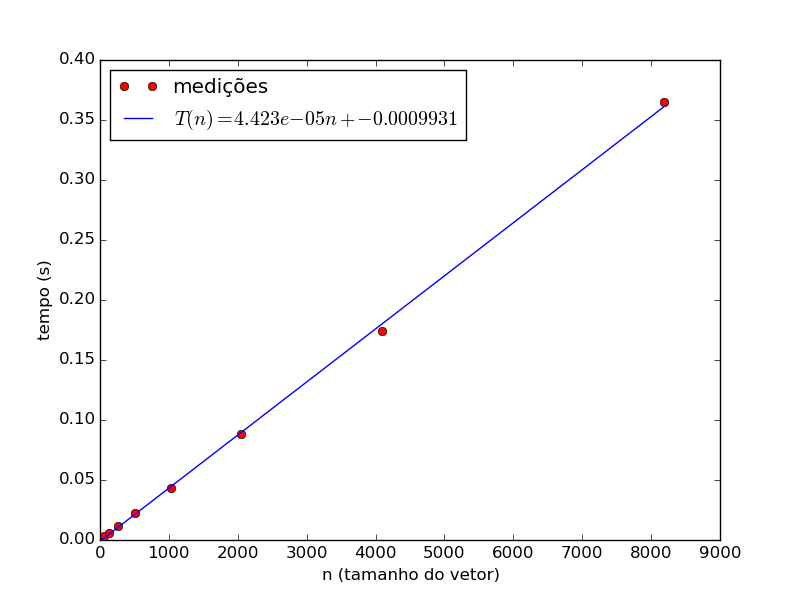
\includegraphics[scale=0.8]{../radixsort/imagens/radixsortQuaseCresc400.png}
\caption{A análise do grafico para $2^{32}$ segue abaixo para radixsort}

Tendo a função $T(n) = 4.423\mathrm{e}-5*n-0.0009931$ e para o $n =2^{32}$, $T(2^{32}) =189966.40250898$
\label{fig:radixsortQuaseCresc400}
\end{figure}

\begin{figure}[ht]
\centering 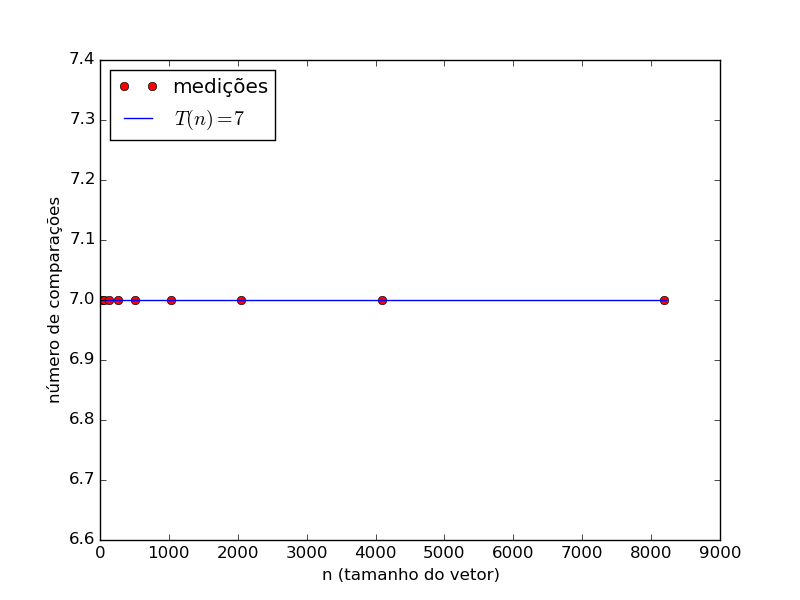
\includegraphics[scale=0.8]{../radixsort/imagens/radixsortQuaseCresc401.png}
\caption{A análise do grafico para $2^{32}$ segue abaixo para radixsort}

Tendo a função $T(n) = 7$ e para o $n =2^{32}$, $T(2^{32}) = 7$
\label{fig:radixsortQuaseCresc401}
\end{figure}


\begin{table}[ht]
\centering
\begin{tabular}{rrr} \toprule
        n &    comparações &       tempo(s) \\ \midrule
      32  &              7 &      0.001634 \\
      64  &              7 &      0.003030 \\
     128  &              7 &      0.006089 \\
     256  &              7 &      0.010584 \\
     512  &              7 &      0.023260 \\
    1024  &              7 &      0.045386 \\
    2048  &              7 &      0.091863 \\
    4096  &              7 &      0.170947 \\
    8192  &              7 &      0.371376 \\
\bottomrule\addlinespace
\end{tabular}
\caption{Tabela com vetor teste quase crecente 50\%: A linha te interesse analisada para este caso é a 16.}
\label{tab:radixsortQuaseCresc50}
\end{table}


\begin{figure}[ht]
\centering 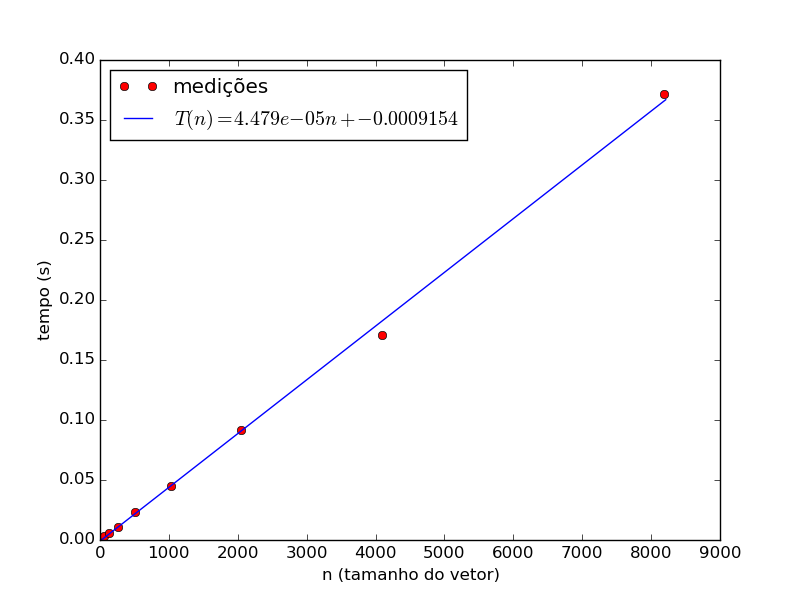
\includegraphics[scale=0.8]{../radixsort/imagens/radixsortQuaseCresc500.png}
\caption{A análise do grafico para $2^{32}$ segue abaixo para radixsort}

Tendo a função $T(n) = 4.479\mathrm{e}-5*n-0.0009154$ e para o $n =2^{32}$, $T(2^{32}) = 192371.58427244$
\label{fig:radixsortQuaseCresc500}
\end{figure}

\begin{figure}[ht]
\centering 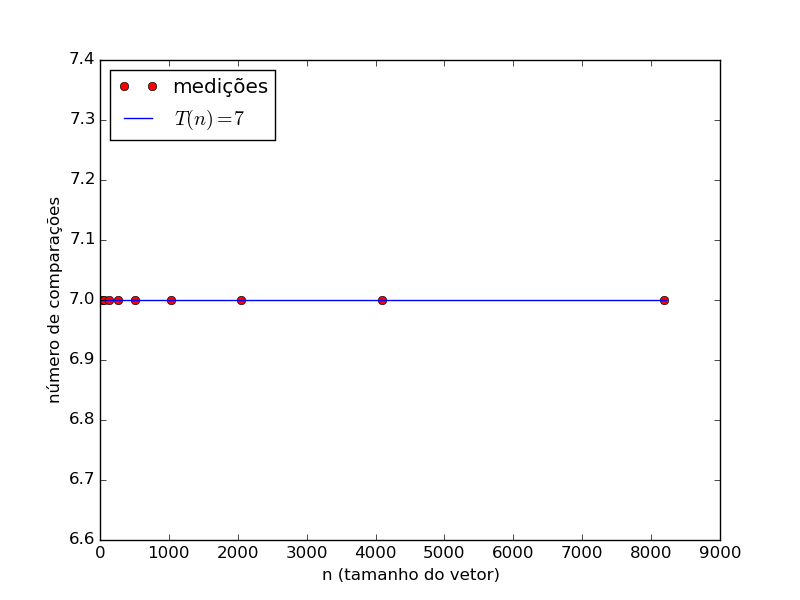
\includegraphics[scale=0.8]{../radixsort/imagens/radixsortQuaseCresc501.png}
\caption{A análise do grafico para $2^{32}$ segue abaixo para radixsort}

Tendo a função $T(n) = 7$ e para o $n =2^{32}$, $T(2^{32}) = 7$
\label{fig:radixsortQuaseCresc501}
\end{figure}


\begin{table}[ht]
\centering
\begin{tabular}{rrr} \toprule
        n &    comparações &       tempo(s) \\ \midrule
      32  &              7 &      0.001529 \\
      64  &              7 &      0.003056 \\
     128  &              7 &      0.005462 \\
     256  &              7 &      0.011047 \\
     512  &              7 &      0.022181 \\
    1024  &              7 &      0.044950 \\
    2048  &              7 &      0.087427 \\
    4096  &              7 &      0.168300 \\
    8192  &              7 &      0.343764 \\
\bottomrule\addlinespace
\end{tabular}
\caption{Tabela com vetor teste quase decrecente 10\%: A linha te interesse analisada para este caso é a 16.}
\label{tab:radixsortQuaseDecresc10}
\end{table}


\begin{figure}[ht]
\centering 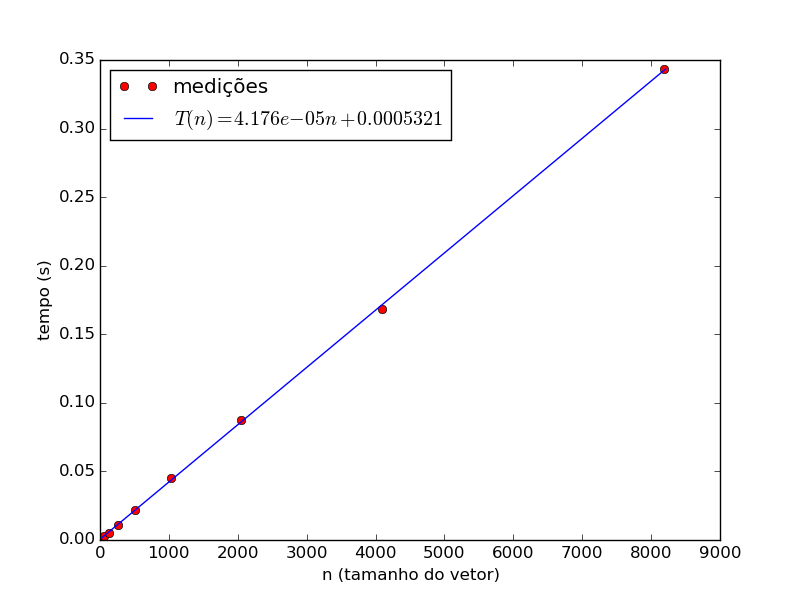
\includegraphics[scale=0.8]{../radixsort/imagens/radixsortQuaseDecresc100.png}
\caption{Explique o gráfico: radixsortQuaseDecresc100.png}
\label{fig:radixsortQuaseDecresc100}
\end{figure}

\begin{figure}[ht]
\centering 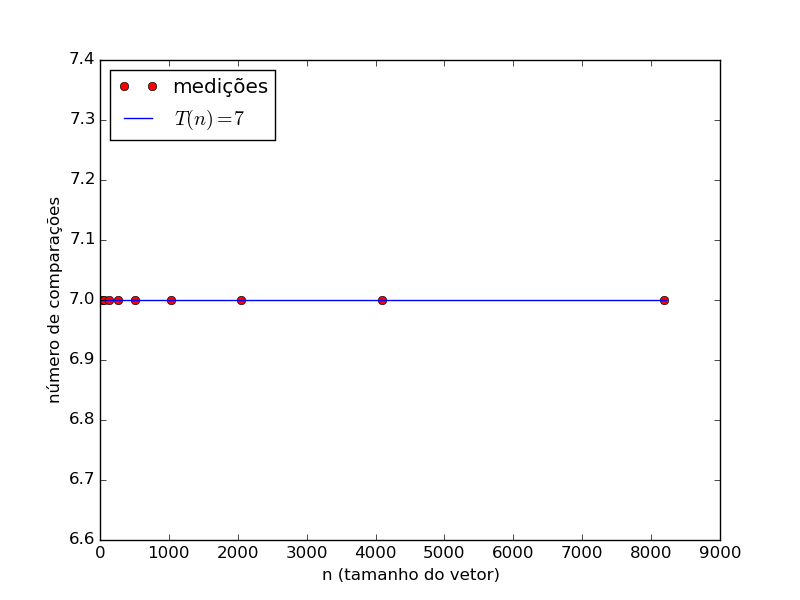
\includegraphics[scale=0.8]{../radixsort/imagens/radixsortQuaseDecresc101.png}
\caption{Explique o gráfico: radixsortQuaseDecresc101.png}
\label{fig:radixsortQuaseDecresc101}
\end{figure}


\begin{table}[ht]
\centering
\begin{tabular}{rrr} \toprule
        n &    comparações &       tempo(s) \\ \midrule
      32  &              7 &      0.001511 \\
      64  &              7 &      0.003001 \\
     128  &              7 &      0.005442 \\
     256  &              7 &      0.010978 \\
     512  &              7 &      0.021155 \\
    1024  &              7 &      0.043353 \\
    2048  &              7 &      0.086680 \\
    4096  &              7 &      0.171603 \\
    8192  &              7 &      0.343652 \\
\bottomrule\addlinespace
\end{tabular}
\caption{Tabela com vetor teste quase decrecente 20\%: A linha te interesse analisada para este caso é a 16.}
\label{tab:radixsortQuaseDecresc20}
\end{table}


\begin{figure}[ht]
\centering 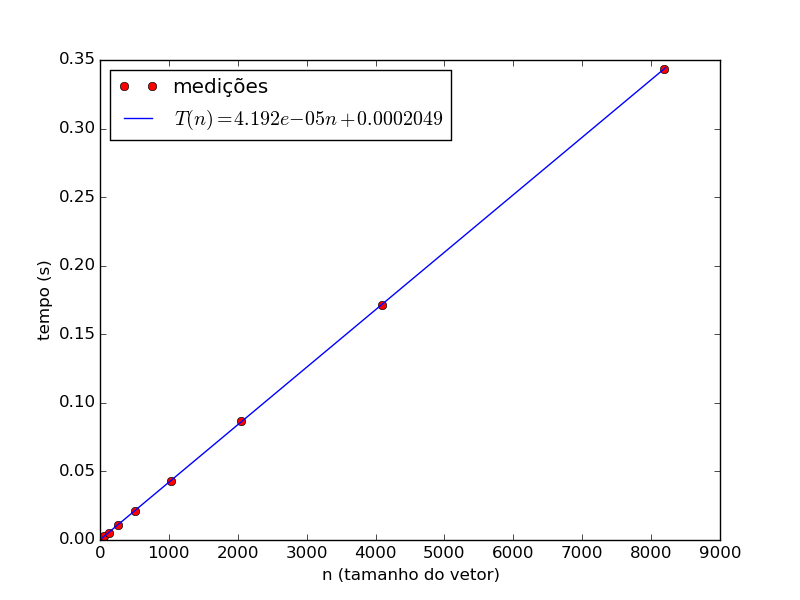
\includegraphics[scale=0.8]{../radixsort/imagens/radixsortQuaseDecresc200.png}
\caption{Explique o gráfico: radixsortQuaseDecresc200.png}
\label{fig:radixsortQuaseDecresc200}
\end{figure}

\begin{figure}[ht]
\centering 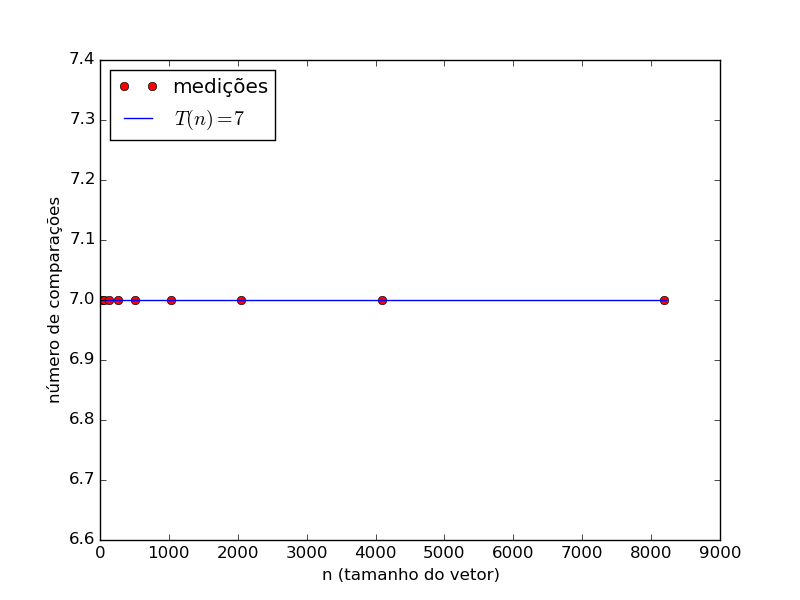
\includegraphics[scale=0.8]{../radixsort/imagens/radixsortQuaseDecresc201.png}
\caption{Explique o gráfico: radixsortQuaseDecresc201.png}
\label{fig:radixsortQuaseDecresc201}
\end{figure}

\clearpage
\begin{table}[ht]
\centering
\begin{tabular}{rrr} \toprule
        n &    comparações &       tempo(s) \\ \midrule
      32  &              7 &      0.001571 \\
      64  &              7 &      0.003061 \\
     128  &              7 &      0.005747 \\
     256  &              7 &      0.011117 \\
     512  &              7 &      0.022279 \\
    1024  &              7 &      0.043290 \\
    2048  &              7 &      0.088795 \\
    4096  &              7 &      0.165978 \\
    8192  &              7 &      0.332857 \\
\bottomrule\addlinespace
\end{tabular}
\caption{Tabela com vetor teste quase decrecente 30\%: A linha te interesse analisada para este caso é a 16.}
\label{tab:radixsortQuaseDecresc30}
\end{table}


\begin{figure}[ht]
\centering 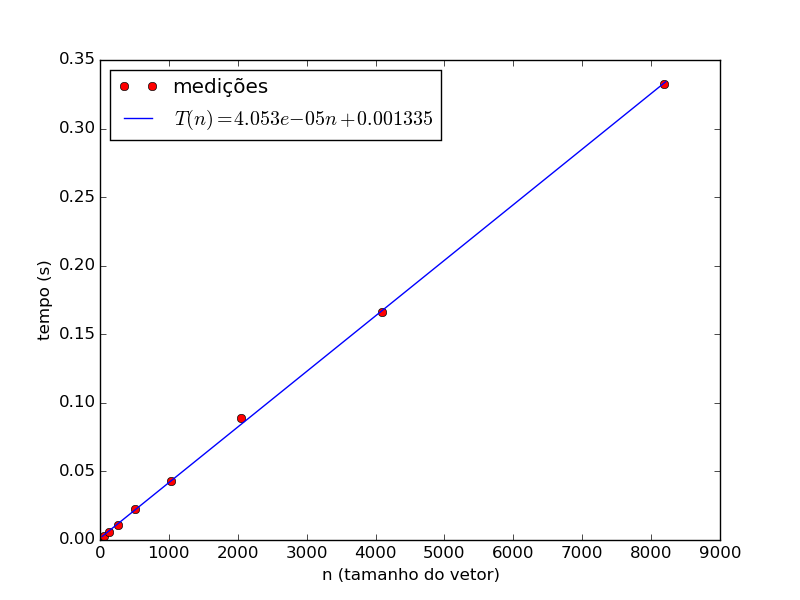
\includegraphics[scale=0.8]{../radixsort/imagens/radixsortQuaseDecresc300.png}
\caption{Explique o gráfico: radixsortQuaseDecresc300.png}
\label{fig:radixsortQuaseDecresc300}
\end{figure}

\begin{figure}[ht]
\centering 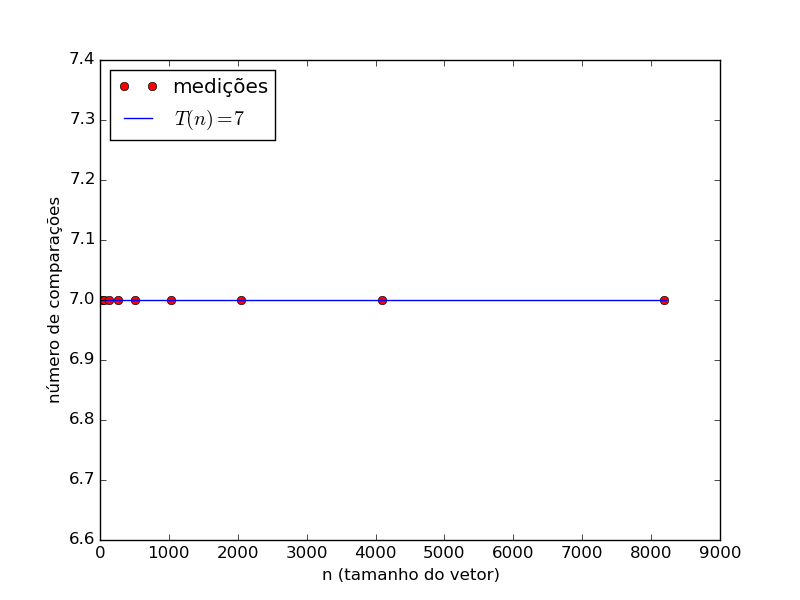
\includegraphics[scale=0.8]{../radixsort/imagens/radixsortQuaseDecresc301.png}
\caption{Explique o gráfico: radixsortQuaseDecresc301.png}
\label{fig:radixsortQuaseDecresc301}
\end{figure}


\begin{table}[ht]
\centering
\begin{tabular}{rrr} \toprule
        n &    comparações &       tempo(s) \\ \midrule
      32  &              7 &      0.001609 \\
      64  &              7 &      0.003027 \\
     128  &              7 &      0.005516 \\
     256  &              7 &      0.011404 \\
     512  &              7 &      0.021144 \\
    1024  &              7 &      0.045238 \\
    2048  &              7 &      0.088607 \\
    4096  &              7 &      0.174904 \\
    8192  &              7 &      0.365459 \\
\bottomrule\addlinespace
\end{tabular}
\caption{Tabela com vetor teste quase decrecente 40\%: A linha te interesse analisada para este caso é a 16.}
\label{tab:radixsortQuaseDecresc40}
\end{table}


\begin{figure}[ht]
\centering 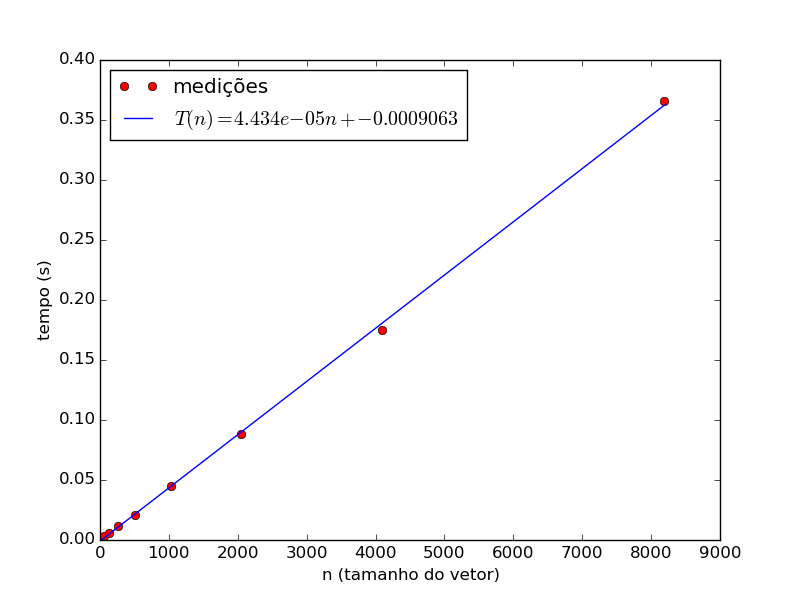
\includegraphics[scale=0.8]{../radixsort/imagens/radixsortQuaseDecresc400.png}
\caption{Explique o gráfico: radixsortQuaseDecresc400.png}
\label{fig:radixsortQuaseDecresc400}
\end{figure}

\begin{figure}[ht]
\centering 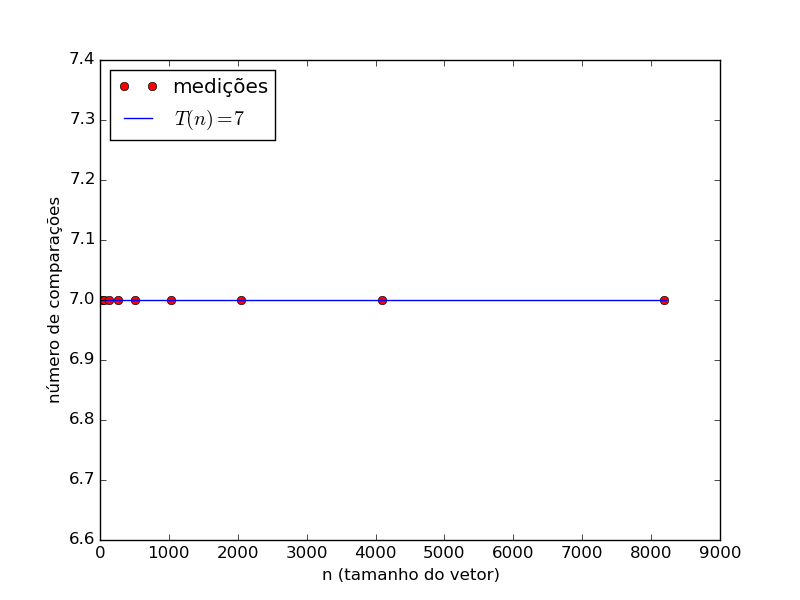
\includegraphics[scale=0.8]{../radixsort/imagens/radixsortQuaseDecresc401.png}
\caption{Explique o gráfico: radixsortQuaseDecresc401.png}
\label{fig:radixsortQuaseDecresc401}
\end{figure}


\begin{table}[ht]
\centering
\begin{tabular}{rrr} \toprule
        n &    comparações &       tempo(s) \\ \midrule
      32  &              7 &      0.001490 \\
      64  &              7 &      0.002849 \\
     128  &              7 &      0.005595 \\
     256  &              7 &      0.010997 \\
     512  &              7 &      0.023139 \\
    1024  &              7 &      0.042961 \\
    2048  &              7 &      0.085150 \\
    4096  &              7 &      0.167020 \\
    8192  &              7 &      0.343861 \\
\bottomrule\addlinespace
\end{tabular}
\caption{Tabela com vetor teste quase decrecente 50\%: A linha te interesse analisada para este caso é a 16.}
\label{tab:radixsortQuaseDecresc50}
\end{table}


\begin{figure}[ht]
\centering 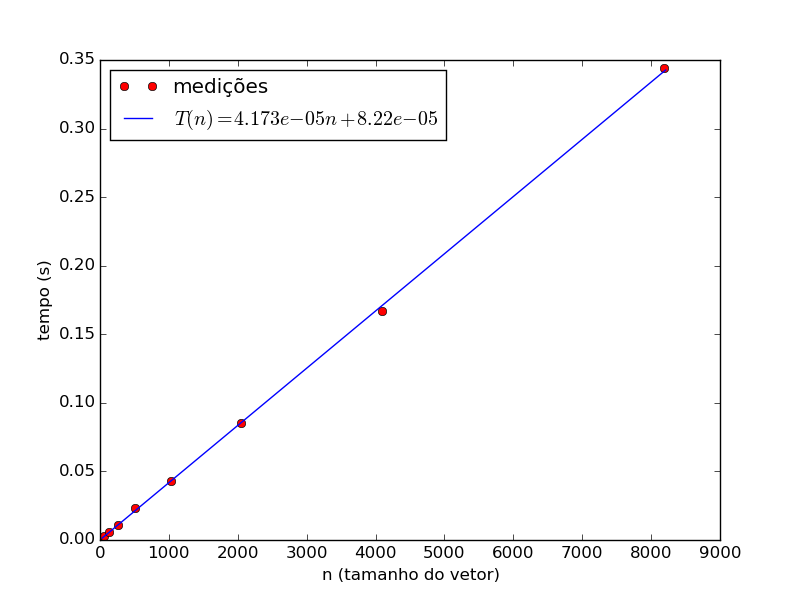
\includegraphics[scale=0.8]{../radixsort/imagens/radixsortQuaseDecresc500.png}
\caption{Explique o gráfico: radixsortQuaseDecresc500.png}
\label{fig:radixsortQuaseDecresc500}
\end{figure}

\begin{figure}[ht]
\centering 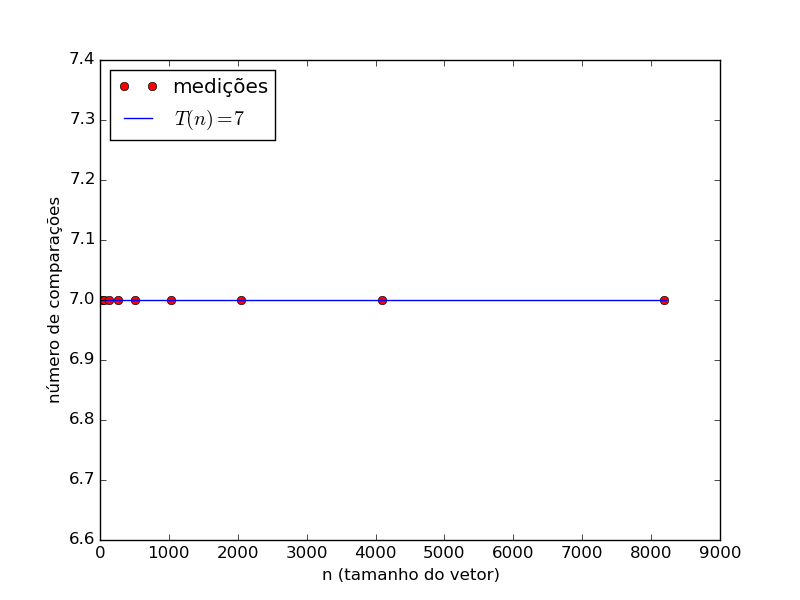
\includegraphics[scale=0.8]{../radixsort/imagens/radixsortQuaseDecresc501.png}
\caption{Explique o gráfico: radixsortQuaseDecresc501.png}
\label{fig:radixsortQuaseDecresc501}
\end{figure}


\clearpage
\clearpage
\addcontentsline{toc}{part}{Apêndice}
\appendix

\chapter{Arquivo ../radixsort/radixsort.py \label{ap:radixsort}}
\lstinputlisting[caption={../radixsort/radixsort.py \label{arq:radixsort}}]{../radixsort/radixsort.py}

\chapter{Arquivo ../radixsort/ensaio.py \label{ap:radixsortensaio}}
\lstinputlisting[caption={../radixsort/ensaio.py \label{arq:radixsortensaio}}]{../radixsort/ensaio.py}

\end{document}
